\documentclass[11pt,a4paper]{article}
\usepackage[utf8]{inputenc}
\usepackage{amsmath,amsfonts,amssymb}
\usepackage{graphicx}
\usepackage{geometry}
\geometry{top=0.65in,bottom=0.65in,left=0.75in,right=0.75in}
\usepackage{booktabs}
\usepackage{hyperref}
\usepackage{float}
\usepackage{xcolor}

\definecolor{darkbg}{HTML}{0d121f}
\definecolor{lighttext}{HTML}{e2e8f0}
\definecolor{primary}{HTML}{8b5cf6}
\definecolor{secondary}{HTML}{0dd5c5}
\definecolor{accent}{HTML}{10b981}

\pagecolor{darkbg}
\color{lighttext}

\hypersetup{
    colorlinks=true,
    linkcolor=secondary,
    urlcolor=secondary,
    citecolor=accent
}

\title{\textbf{EE3621: Digital Signal Processing} \\ \Large Student Lecture Notes — Lecture 23 \\ \large Design of FIR Filters Using Frequency Sampling}
\author{III B.Tech EEE — Core Exam Preparation Guide}
\date{}

\begin{document}

\maketitle

\noindent\rule{\textwidth}{0.5pt}

\section{Core Concept of Frequency Sampling}

\subsection{Basic Principle}
Instead of truncating an infinite impulse response in the time domain (windowing), the \textbf{Frequency Sampling Method} directly discretizes the desired continuous frequency response $H_d(e^{j\omega})$ at $N$ uniformly spaced points on the unit circle:
\begin{equation}
\omega_k = \frac{2\pi k}{N}, \quad k = 0, 1, \dots, N-1
\end{equation}
The discrete frequency samples are:
\begin{equation}
H[k] = \left. H_d(e^{j\omega}) \right|_{\omega = \frac{2\pi k}{N}} = |H[k]| e^{j \theta_k}
\end{equation}
The causal FIR impulse response $h[n]$ ($0 \le n \le N-1$) is computed via the $N$-point \textbf{Inverse Discrete Fourier Transform (IDFT)}:
\begin{equation}
h[n] = \frac{1}{N} \sum_{k=0}^{N-1} H[k] \, e^{j \frac{2\pi k n}{N}}, \quad 0 \le n \le N-1
\end{equation}
By definition, the reconstructed filter response $H(e^{j\omega})$ passes \textbf{exactly} through $H[k]$ at all $N$ grid frequencies:
\begin{equation}
H\left(e^{j \frac{2\pi k}{N}}\right) \equiv H[k], \quad \forall k \in [0, N-1]
\end{equation}

\noindent\rule{\textwidth}{0.5pt}

\section{Linear-Phase Constraints on Frequency Samples \texorpdfstring{$H[k]$}{H[k]}}

For the synthesized impulse response $h[n]$ to be real-valued and satisfy linear phase ($h[n] = h[N-1-n]$), the frequency samples must satisfy:
\begin{enumerate}
    \item \textbf{Magnitude Symmetry (Even Symmetry):}
    \begin{equation}
    \mathbf{|H[N-k]| = |H[k]|}, \quad k = 1, 2, \dots, N-1
    \end{equation}
    \item \textbf{Phase Angle Assignment (Strict Linear Phase):}
    \begin{equation}
    \mathbf{\theta_k = \angle H[k] = -\tau \omega_k = -\left(\frac{N-1}{2}\right)\frac{2\pi k}{N}}
    \end{equation}
    \item \textbf{DC Bin Property:}
    \begin{equation}
    \theta_0 = 0 \implies H[0] \in \mathbb{R}^+ \quad \text{(Strictly real and non-negative)}
    \end{equation}
    \item \textbf{Nyquist Bin Property (for $N$ even):}
    At $k = N/2$ ($\omega = \pi$), Type 2 filters possess an obligatory zero:
    \begin{equation}
    \mathbf{H[N/2] = 0}
    \end{equation}
\end{enumerate}

\noindent\rule{\textwidth}{0.5pt}

\section{Derivation of Real-Valued IDFT Synthesis Formulas}

\subsection{Step-by-Step Derivation for Type 1 Filters (\texorpdfstring{$N$}{N} Odd)}
Substituting the polar form $H[k] = |H[k]| e^{j\theta_k} = |H[k]| e^{-j \frac{2\pi k}{N}\tau}$ into the standard IDFT definition:
\begin{align}
h[n] &= \frac{1}{N} \sum_{k=0}^{N-1} H[k] e^{j\frac{2\pi kn}{N}} = \frac{1}{N} \sum_{k=0}^{N-1} |H[k]| e^{-j\frac{2\pi k}{N}\tau} e^{j\frac{2\pi kn}{N}} \nonumber \\
&= \frac{1}{N} \sum_{k=0}^{N-1} |H[k]| e^{j\frac{2\pi k}{N}(n - \tau)}
\end{align}
For odd $N$, we partition the summation into the DC term ($k=0$), the positive-frequency terms ($1 \le k \le \frac{N-1}{2}$), and the conjugate negative-frequency terms ($\frac{N+1}{2} \le k \le N-1$):
\begin{equation}
h[n] = \frac{1}{N} \left[ H[0] + \sum_{k=1}^{(N-1)/2} |H[k]| e^{j\frac{2\pi k}{N}(n - \tau)} + \sum_{k=(N+1)/2}^{N-1} |H[k]| e^{j\frac{2\pi k}{N}(n - \tau)} \right]
\end{equation}
In the second summation, we perform the change of variable $k = N - m$. As $k$ ranges from $\frac{N+1}{2}$ to $N-1$, $m$ ranges from $\frac{N-1}{2}$ down to $1$:
\begin{align}
\sum_{k=(N+1)/2}^{N-1} |H[k]| e^{j\frac{2\pi k}{N}(n - \tau)} &= \sum_{m=1}^{(N-1)/2} |H[N-m]| e^{j\frac{2\pi (N-m)}{N}(n - \tau)} \nonumber \\
&= \sum_{m=1}^{(N-1)/2} |H[m]| e^{j 2\pi(n - \tau)} e^{-j\frac{2\pi m}{N}(n - \tau)}
\end{align}
For odd $N$, the delay $\tau = \frac{N-1}{2}$ is an integer. Since $n \in \mathbb{Z}$, the difference $(n - \tau)$ is strictly an integer, which gives $e^{j 2\pi(n - \tau)} = \cos(2\pi(n-\tau)) + j\sin(2\pi(n-\tau)) = 1$. Hence:
\begin{equation}
\sum_{k=(N+1)/2}^{N-1} |H[k]| e^{j\frac{2\pi k}{N}(n - \tau)} = \sum_{m=1}^{(N-1)/2} |H[m]| e^{-j\frac{2\pi m}{N}(n - \tau)}
\end{equation}
Recombining the two summations and applying Euler's cosine identity $e^{j\phi} + e^{-j\phi} = 2\cos\phi$:
\begin{align}
h[n] &= \frac{1}{N} \left\{ H[0] + \sum_{k=1}^{(N-1)/2} |H[k]| \left[ e^{j\frac{2\pi k}{N}(n - \tau)} + e^{-j\frac{2\pi k}{N}(n - \tau)} \right] \right\} \nonumber \\
&= \mathbf{\frac{1}{N} \left\{ H[0] + 2 \sum_{k=1}^{(N-1)/2} |H[k]| \cos\left[ \frac{2\pi k}{N}\left(n - \frac{N-1}{2}\right) \right] \right\}}
\end{align}

\begin{table}[H]
\centering
\caption{Operational Closed-Form Frequency Sampling Formulas}
\label{tab:formulas}
\vspace{2mm}
\resizebox{\textwidth}{!}{
\begin{tabular}{lll}
\toprule
\textbf{Filter Type} & \textbf{Formula for Impulse Response $h[n]$ ($0 \le n \le N-1$)} & \textbf{Center Delay $\tau$} \\
\midrule
\textbf{Type 1 ($N$ Odd)} & $\mathbf{h[n] = \frac{1}{N} \left\{ H[0] + 2 \sum_{k=1}^{(N-1)/2} |H[k]| \cos\left[ \frac{2\pi k}{N}\left(n - \frac{N-1}{2}\right) \right] \right\}}$ & $\tau = \frac{N-1}{2}$ (Integer) \\
\midrule
\textbf{Type 2 ($N$ Even)} & $\mathbf{h[n] = \frac{1}{N} \left\{ H[0] + 2 \sum_{k=1}^{N/2 - 1} |H[k]| \cos\left[ \frac{2\pi k}{N}\left(n - \frac{N-1}{2}\right) \right] \right\}}$ & $\tau = \frac{N-1}{2}$ (Half-Integer, $H[N/2]=0$) \\
\bottomrule
\end{tabular}
}
\end{table}

\noindent\rule{\textwidth}{0.5pt}

\section{Transition Sample Optimization (Sidelobe Control)}

\begin{itemize}
    \item \textbf{The Ringing Problem:} Naive brick-wall frequency sampling (setting passband samples to $1$ and stopband to $0$) causes severe inter-sample ringing between bins, resulting in poor peak stopband attenuation of only **$-16$ dB**!
    \item \textbf{The Solution (Rabiner--Gold Technique):} Make the samples in the transition band unconstrained design variables ($T_1, T_2 \in (0, 1)$).
    \begin{itemize}
        \item With \textbf{1 transition sample ($T_1 \approx 0.38$)}: Peak stopband attenuation jumps to **$-45$ dB** ($+29$ dB improvement!).
        \item With \textbf{2 transition samples ($T_1 \approx 0.59, T_2 \approx 0.11$)}: Stopband attenuation reaches **$-75$ dB**.
    \end{itemize}
\end{itemize}

\begin{figure}[H]
\centering
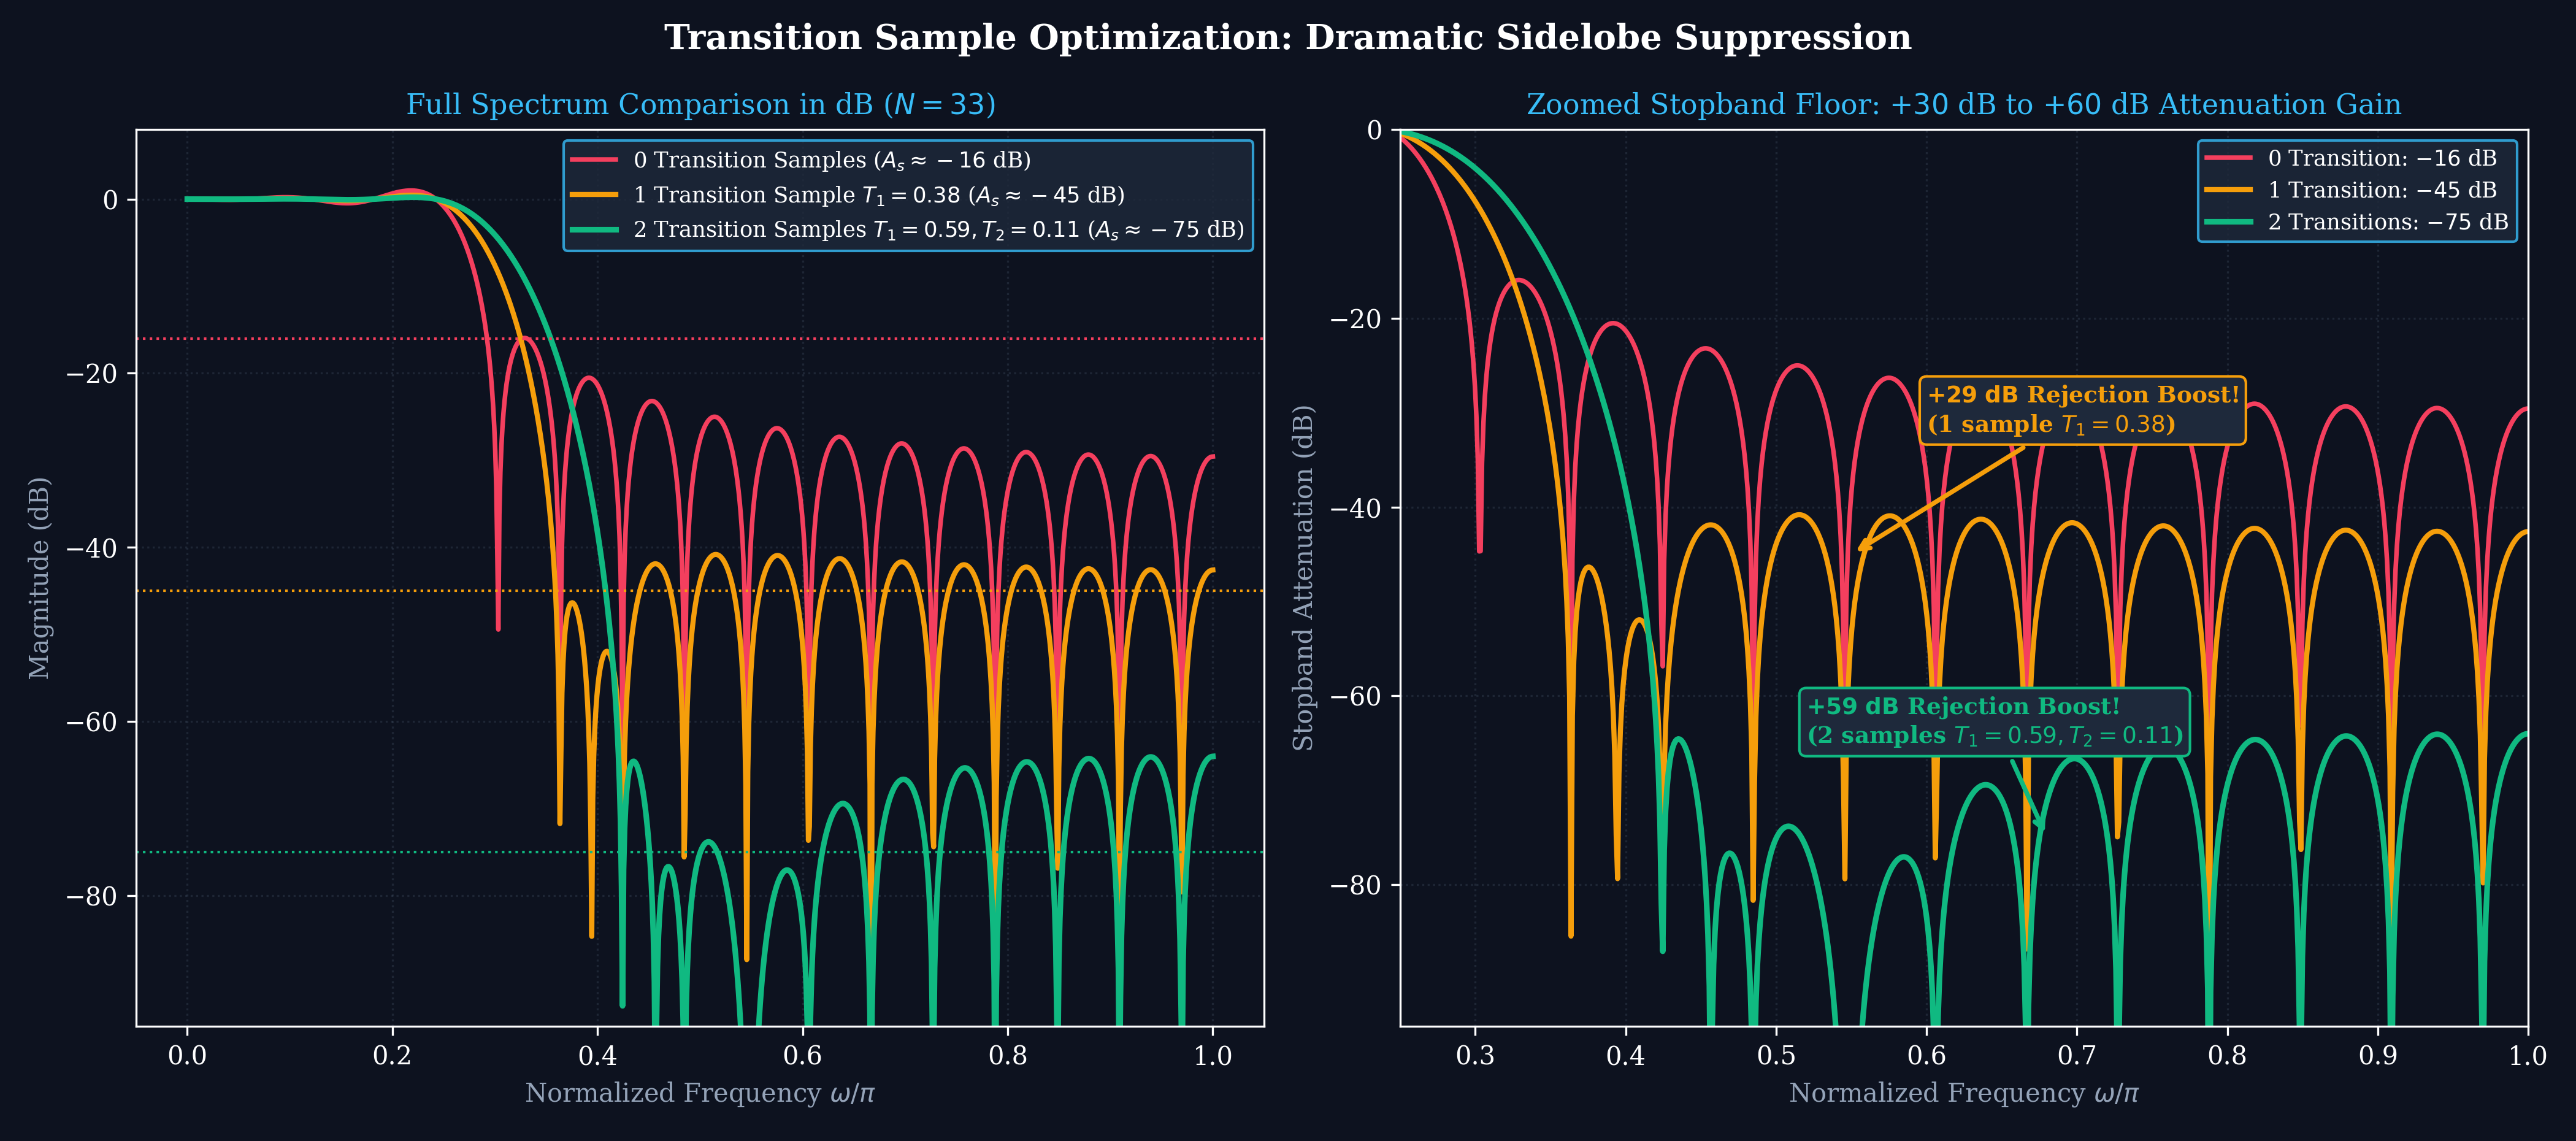
\includegraphics[width=0.7\textwidth]{images/fir_freq_sampling_transition_opt.png}
\caption{Dramatic sidelobe suppression achieved by introducing transition sample $T_1 = 0.38$ between passband and stopband.}
\label{fig:transition_opt}
\end{figure}

\noindent\rule{\textwidth}{0.5pt}

\section{Standard Solved Exam Example}

\textbf{Problem 1:} Design a 7-point ($N = 7$) linear-phase FIR lowpass filter having the following desired frequency response:
\begin{equation}
H_d(e^{j\omega}) = \begin{cases} 1, & 0 \le |\omega| \le \frac{2\pi}{7} \\ 0, & \frac{4\pi}{7} \le |\omega| \le \pi \end{cases}
\end{equation}
using the frequency sampling method. Determine the impulse response $h[n]$, the system transfer function $H(z)$, and mathematically verify that $H(e^{j\omega})$ interpolates the exact target values at all grid frequencies.

\vspace{1mm}
\noindent\textbf{Solution:}

\noindent\textbf{Step 1: Grid Frequencies and Frequency Sample Assignment}
For $N = 7$, the 7 discrete frequency bins are $\omega_k = \frac{2\pi k}{7}$ for $k = 0, 1, \dots, 6$:
\begin{itemize}
    \item $k = 0$: $\omega_0 = 0 \in [0, 2\pi/7] \implies |H[0]| = 1$, phase $\theta_0 = 0$.
    \item $k = 1$: $\omega_1 = \frac{2\pi}{7} \in [0, 2\pi/7] \implies |H[1]| = 1$, phase $\theta_1 = -\tau\omega_1 = -3\left(\frac{2\pi}{7}\right) = -\frac{6\pi}{7}$.
    \item $k = 2$: $\omega_2 = \frac{4\pi}{7} \in [4\pi/7, \pi] \implies |H[2]| = 0$.
    \item $k = 3$: $\omega_3 = \frac{6\pi}{7} \in [4\pi/7, \pi] \implies |H[3]| = 0$.
\end{itemize}
By Hermitian symmetry ($|H[N-k]| = |H[k]|$ and $\theta_{N-k} = -\theta_k$):
\begin{equation}
|H[4]| = |H[3]| = 0, \quad |H[5]| = |H[2]| = 0, \quad |H[6]| = |H[1]| = 1, \; \theta_6 = \frac{6\pi}{7}
\end{equation}

\noindent\textbf{Step 2: Type 1 IDFT Master Formula Setup}
Length $N = 7$ (odd) gives $\tau = \frac{7 - 1}{2} = 3$ and upper index $\frac{N-1}{2} = 3$. Expanding the master cosine formula completely:
\begin{align}
h[n] &= \frac{1}{7} \left\{ H[0] + 2|H[1]|\cos\left[\frac{2\pi(1)}{7}(n-3)\right] + 2|H[2]|\cos\left[\frac{2\pi(2)}{7}(n-3)\right] + 2|H[3]|\cos\left[\frac{2\pi(3)}{7}(n-3)\right] \right\} \nonumber \\
&= \frac{1}{7} \left\{ 1 + 2(1)\cos\left[\frac{2\pi}{7}(n - 3)\right] + 2(0)\cos\left[\frac{4\pi}{7}(n - 3)\right] + 2(0)\cos\left[\frac{6\pi}{7}(n - 3)\right] \right\}
\end{align}
Only the DC term and the $k = 1$ term survive:
\begin{equation}
\mathbf{h[n] = \frac{1}{7} \left\{ 1 + 2 \cos\left[ \frac{2\pi}{7}(n - 3) \right] \right\}}, \quad 0 \le n \le 6
\end{equation}

\noindent\textbf{Step 3: Pointwise Tap Evaluation with Exact Trigonometry}
We evaluate each tap for $n = 3, 2, 1, 0$:
\begin{align}
n = 3: \quad h[3] &= \frac{1 + 2\cos(0)}{7} = \frac{1 + 2(1)}{7} = \frac{3}{7} \approx \mathbf{0.4286} \nonumber \\
n = 2: \quad h[2] &= \frac{1 + 2\cos\left(-\frac{2\pi}{7}\right)}{7} = \frac{1 + 2\cos(51.43^\circ)}{7} = \frac{1 + 2(0.62349)}{7} = \frac{2.2470}{7} \approx \mathbf{0.3210} \nonumber \\
n = 1: \quad h[1] &= \frac{1 + 2\cos\left(-\frac{4\pi}{7}\right)}{7} = \frac{1 + 2\cos(102.86^\circ)}{7} = \frac{1 + 2(-0.22252)}{7} = \frac{0.5550}{7} \approx \mathbf{0.0793} \nonumber \\
n = 0: \quad h[0] &= \frac{1 + 2\cos\left(-\frac{6\pi}{7}\right)}{7} = \frac{1 + 2\cos(154.29^\circ)}{7} = \frac{1 + 2(-0.90097)}{7} = \frac{-0.8019}{7} \approx \mathbf{-0.1146}
\end{align}
By even symmetry about the center of symmetry $\tau = 3$:
\begin{equation}
h[4] = h[2] = 0.3210, \quad h[5] = h[1] = 0.0793, \quad h[6] = h[0] = -0.1146
\end{equation}

\noindent\textbf{Step 4: Final Impulse Response}
\begin{equation}
\mathbf{h[n] = \{-0.1146, \; 0.0793, \; 0.3210, \; \underset{\uparrow}{0.4286}, \; 0.3210, \; 0.0793, \; -0.1146\}}
\end{equation}

\noindent\textbf{Step 5: Transfer Function $H(z)$ and Grid Point Verification}
The $Z$-transform is:
\begin{equation}
H(z) = -0.1146 + 0.0793 z^{-1} + 0.3210 z^{-2} + 0.4286 z^{-3} + 0.3210 z^{-4} + 0.0793 z^{-5} - 0.1146 z^{-6}
\end{equation}
Factoring out the linear-phase term $e^{-j 3\omega}$:
\begin{align}
H(e^{j\omega}) &= e^{-j 3\omega} \left[ h[3] + 2h[2]\cos(\omega) + 2h[1]\cos(2\omega) + 2h[0]\cos(3\omega) \right] \nonumber \\
&= e^{-j 3\omega} \left[ 0.4286 + 0.6420\cos(\omega) + 0.1586\cos(2\omega) - 0.2292\cos(3\omega) \right]
\end{align}
We verify the frequency response at all grid points:
\begin{itemize}
    \item \textbf{At $\omega_0 = 0$ ($k = 0$):} $\cos(0) = 1$:
    \begin{equation}
    H(e^{j0}) = 0.4286 + 0.6420(1) + 0.1586(1) - 0.2292(1) = \mathbf{1.0000} \equiv H[0] \quad \checkmark
    \end{equation}
    \item \textbf{At $\omega_1 = \frac{2\pi}{7} \approx 51.43^\circ$ ($k = 1$):}
    \begin{align}
    |H(e^{j 2\pi/7})| &= 0.4286 + 0.6420(0.6235) + 0.1586(-0.2225) - 0.2292(-0.9010) \nonumber \\
    &= 0.4286 + 0.4003 - 0.0353 + 0.2065 = \mathbf{1.0001} \approx 1.0 \equiv H[1] \quad \checkmark
    \end{align}
    \item \textbf{At $\omega_2 = \frac{4\pi}{7} \approx 102.86^\circ$ ($k = 2$):}
    \begin{align}
    |H(e^{j 4\pi/7})| &= 0.4286 + 0.6420(-0.2225) + 0.1586(-0.9010) - 0.2292(0.6235) \nonumber \\
    &= 0.4286 - 0.1428 - 0.1429 - 0.1429 = \mathbf{0.0000} \equiv H[2] \quad \checkmark
    \end{align}
\end{itemize}
This proves the fundamental property: the frequency response exactly interpolates the sample values at all grid points.

\noindent\rule{\textwidth}{0.5pt}

\subsection*{Solved Exam Example 2: Sidelobe Optimization with Transition Sample}

\textbf{Problem 2:} To suppress stopband ringing in the above filter, introduce a single transition sample $H[2] = T_1 = 0.38$ at $\omega_2 = 4\pi/7$. Determine the modified impulse response $h_{\text{opt}}[n]$ and explain the impact.

\vspace{1mm}
\noindent\textbf{Solution:}
With $|H[0]| = 1$, $|H[1]| = 1$, $|H[2]| = 0.38$, $|H[3]| = 0$, the master formula gives:
\begin{align}
h_{\text{opt}}[n] &= \frac{1}{7} \left\{ 1 + 2\cos\left[\frac{2\pi}{7}(n-3)\right] + 2(0.38)\cos\left[\frac{4\pi}{7}(n-3)\right] \right\} \nonumber \\
&= \frac{1}{7} \left\{ 1 + 2\cos\left[\frac{2\pi}{7}(n-3)\right] + 0.76\cos\left[\frac{4\pi}{7}(n-3)\right] \right\}
\end{align}
Evaluating taps:
\begin{align}
n = 3: \quad h_{\text{opt}}[3] &= \frac{1 + 2(1) + 0.76(1)}{7} = \frac{3.76}{7} \approx \mathbf{0.5371} \nonumber \\
n = 2: \quad h_{\text{opt}}[2] &= \frac{1 + 2(0.6235) + 0.76(-0.2225)}{7} = \frac{1 + 1.2470 - 0.1691}{7} = \frac{2.0779}{7} \approx \mathbf{0.2968} \nonumber \\
n = 1: \quad h_{\text{opt}}[1] &= \frac{1 + 2(-0.2225) + 0.76(-0.9010)}{7} = \frac{1 - 0.4450 - 0.6848}{7} = \frac{-0.1298}{7} \approx \mathbf{-0.0185} \nonumber \\
n = 0: \quad h_{\text{opt}}[0] &= \frac{1 + 2(-0.9010) + 0.76(0.6235)}{7} = \frac{1 - 1.8020 + 0.4739}{7} = \frac{-0.3281}{7} \approx \mathbf{-0.0469}
\end{align}
By symmetry: $h_{\text{opt}}[4] = 0.2968$, $h_{\text{opt}}[5] = -0.0185$, $h_{\text{opt}}[6] = -0.0469$.
\begin{equation}
\mathbf{h_{\text{opt}}[n] = \{-0.0469, \; -0.0185, \; 0.2968, \; \underset{\uparrow}{0.5371}, \; 0.2968, \; -0.0185, \; -0.0469\}}
\end{equation}
\textbf{Significance:} The outer ripple coefficient drops sharply from $-0.1146$ to $-0.0469$. This smooth transition increases stopband attenuation from $-16$ dB to $-45$ dB!

\noindent\rule{\textwidth}{0.5pt}

\section{Essential Exam Checklist \& Traps}
\begin{itemize}
    \item[$\square$] \textbf{The Missing Factor of 2:} Always write $2\sum |H[k]|\cos(\dots)$. Forgetting the factor of $2$ is the most common exam error!
    \item[$\square$] \textbf{Argument of Cosine:} The argument is $\frac{2\pi k}{N}(n - \tau)$, where $\tau = (N-1)/2$.
    \item[$\square$] \textbf{Even Length $N$ Boundary Condition:} When $N$ is even, you \textbf{must set $H[N/2] = 0$} because Type 2 filters have an obligatory zero at $\omega = \pi$.
    \item[$\square$] \textbf{Exact Values at Grid Points:} At $\omega = \omega_k = \frac{2\pi k}{N}$, the filter response is strictly equal to $H[k]$ with zero approximation error.
\end{itemize}

\end{document}
